\section[Lezione 9 - Metodo di Newton]{Lezione 9 - Metodo di Newton (tangenti), convergenza e velocità di convergenza}
\subsection{Velocità di convergenza metodo di bisezione}
Come abbiamo visto nella scorsa lezione, il metodo di bisezione è un metodo semplice ed efficace per la soluzione numerica di equazioni non lineari, in grado di funzionare con richieste minimali, sia dal punto di vista analitico (ipotesi del teorema degli zeri delle funzioni continue) sia computazionali (basta saper calcolare il segno di $f(x_n)$ cioè fare su $f(x_n)$ un errore relativo $<100\%$).\\
Accanto a questi indubbi vantaggi, il metodo di bisezione ha però un handicap: è abbastanza ``lento". Come abbiamo visto, la stima a priori dell'errore decade di un fattore $\frac{1}{2}$ ad ogni iterazione e l'errore lo fa ``in media", cioè 
\[ e_{n+1} \approx \frac{1}{2} \cdot e_n \]
non esattamente ad ogni iterazione ma in media su un certo numero di iterazioni.\\
Ovviamente la stessa proprietà vale in media per l'errore relativo
\[ r_{n+1}=\frac{e_{n+1}}{\abs{\,\xi\,}} \approx \frac{1}{2} \cdot \frac{e_n}{\abs{\,\xi\,}} = \frac{1}{2} \cdot r_n \]
per $\xi \ne 0$; sono quindi necessarie in media $3-4$ iterazioni affinché l'errore relativo scenda di $\frac{1}{10}$ (cioè per guadagnare una cifra decimale corretta), visto che 
\[\frac{1}{16} = \left(\frac{1}{2}\right)^4 < \frac{1}{10} < \left(\frac{1}{2}\right)^3 = \frac{1}{8}\] 
(infatti abbiamo visto che per calcolare $\sqrt{2}$ alla precisione di macchina in Matlab servono una cinquantina di iterazioni e in effetti $\varepsilon_M = 2^{-53} \approx 10^{-16}$).

\subsection{Metodo di Newton}
In queste lezioni introdurremo un metodo molto più efficiente per il calcolo di zeri, ovvero il metodo di \uline{Newton}, o metodo delle \uline{tangenti}, che come si capisce dal nome risale agli albori del calcolo differenziale nel XVII secolo.\\
La maggior efficienza avrà un prezzo in termini di richieste analitiche ($f$ almeno derivabile in $[a, b]$) e computazionali (saper calcolare sia $f$ che $f'$ con buona accuratezza).\\
L'idea del metodo è semplice: si tratta di \uline{LINEARIZZARE} iterativamente l'equazione $f(x) = 0$ sostituendo $f$ ad ogni iterazione con la retta tangente nel punto ($x_n, f(x_n)$) del grafico (purché $f$ sia derivabile), come vediamo nel disegno qui sotto 
\begin{center}
    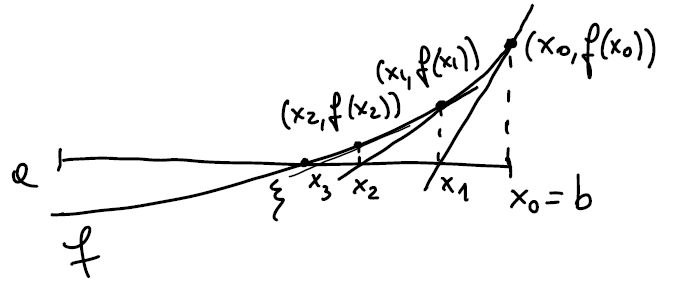
\includegraphics[scale=0.7]{foto/pagina5_1}
\end{center}
Per trovare l'espressione analitica delle iterazioni, calcoliamo lo zero della retta tangente nel punto($x_0,f(x_0)$):
\[ \begin{cases}
    y = 0 & \text{asse } x\\
    y = f(x_0) + f'(x_0)(x-x_0) & \text{retta tangente}
\end{cases}\]
dove stiamo usando l'interpretazione geometrica della derivata nel punto $x_0$ come coefficiente angolare della retta tangente nel corrispondente punto del grafico di $f$. Otteniamo l'equazione 
\[ 0=f(x_0)+ f'(x_0)(x-x_0) \]
la cui soluzione è
\[ x_1=x_0-\frac{f(x_0)}{f'(x_0)}, \quad f'(x_0)\neq 0 \]
Osserviamo subito che se $f'(x_0)=0$ la retta tangente sarebbe parallela all'asse $x$ e non avrebbe un punto di intersezione con esso; ma è essenziale anche la posizione del valore iniziale $x_0$, se scelto ``male" già la prima iterazione potrebbe far uscire dall'intervallo di definizione:\\
\begin{center}
    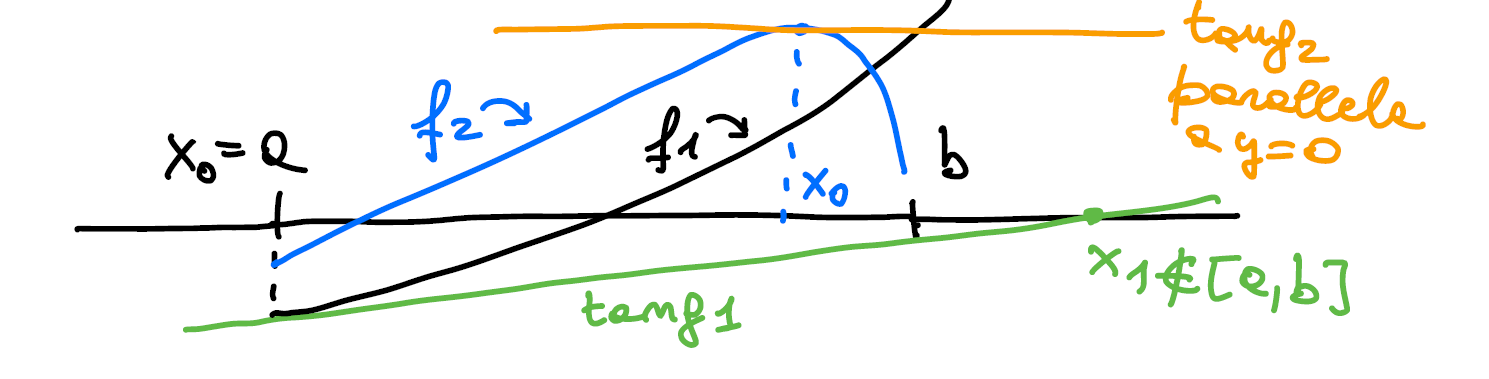
\includegraphics[scale=0.5]{foto/pagina7}
\end{center}
In generale, per ottenere $x_{n+1}$ a partire da $x_n$ (se $f'(x_n)\neq 0$) si cerca l'intersezione della tangente in ($x_n,f(x_n)$ con l'asse $x$ ($y=0$)\\
\[ \begin{cases}
        y=0\\
        y=f(x_n)+f'(x_n)(x-x_n)
\end{cases} \]
ottenendo la formula iterativa\\
\[ x_{n+1}=x_n-\frac{f(x_n)}{f'(x_n)}, \quad n=0,1,2,\dotso \]
Ora, come per tutti i metodi che producano una successione, cerchiamo delle condizioni che garantiscano la CONVERGENZA (in questo caso il limite dovrà essere lo zero $\xi$ di $f$).\\
Ci sono vari set di condizioni SUFFICIENTI che garantiscono la convergenza del metodo di Newton; ne mostriamo uno che assume, oltre alle ipotesi del teorema degli zeri, la derivabilità (essenziale perché la curva del grafico ammetta tangente in ogni punto) e la convessità o concavità stretta (tramite il segno di $f''$).

\subsubsection{TEOREMA (convergenza del metodo di Newton con $f''$ segno costante)}
\begin{center}
    \fbox{\begin{minipage}[t]{15cm}%
            Sia $f \in C^2[a,b]$ (derivabile 2 volte con derivate continue in $[a,b]$), $f(a)f(b)<0$, $f''(x)>0 \quad \forall x \in [a,b]$ (oppure $f''(x)<0 \quad \forall x \in [a,b]$), $x_0$ tali che $f(x_0)f''(x_0)>0$
        allora 
        \begin{center}
        il metodo di Newton è ben definito (cioè $f'(x_n) \neq 0 \ \ \forall n$)\\
        e converge all'unico zero $\xi$ di $f$ in $(a,b)$
        \end{center}
    \end{minipage}}
\end{center}
\begin{proof}[\unskip\nopunct]
\textbf{Dimostrazione}\\
Ci sono 4 casi possibili in base al segno di $f''$ ovvero
\begin{center}
    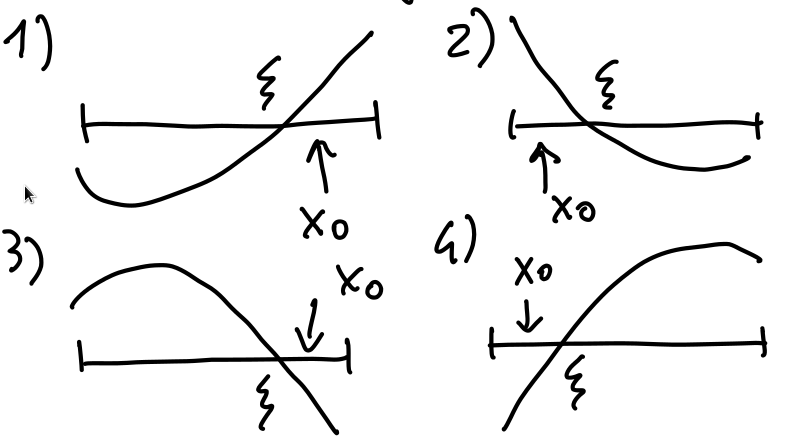
\includegraphics[scale=0.4]{foto/pagina11_1}
\end{center}
\begin{itemize}
    \item in (1) e (2) $f$ è strettamente convessa,
    \item in (3) e (4) concava,
    \item in (1) e (3) $x_0$ va scelto in $(\xi,b]$,
    \item in (2) e (4) $x_0 $ va scelto in $[a,\xi)$.
\end{itemize}
Vediamo dai disegni che non è escluso che $f'$ possa cambiare segno, l'ipotesi chiave è che non cambi segno $f''$; ovviamente sono compresi i casi in cui $f''$ non cambia segno e anche $f'$ non lo fa, ad esempio $f''(x) > 0$ e $f'(x) > 0 \quad \forall x \in [a,b]$, cioè $f$ è strettamente convessa e strettamente crescente in [a,b], tipo\\
\begin{center}
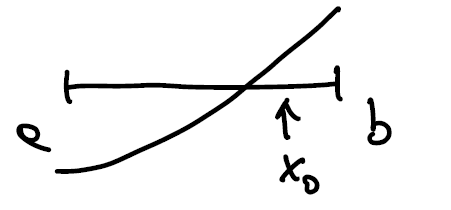
\includegraphics[width=0.3\textwidth]{foto/pagina12_1}
\end{center}
Per semplicità trattiamo il caso (1) perché negli altri casi la dimostrazione è analoga. \\
Siamo quindi in questa situazione\\
\begin{center}
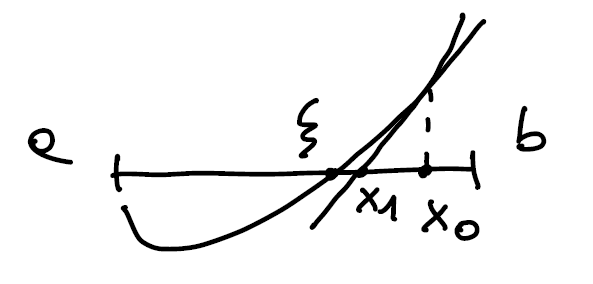
\includegraphics[width=0.3\textwidth]{foto/pagina12_2}
\end{center}
con $f(a) < 0$, $f(b) > 0$, $f''(x) > 0$, $\forall x \in [a,b]$, $x_0 \in (\xi,b]$\\
La dimostrazione si fa per induzione, mostrando che se $x_n \in (\xi, b]$ anche $x_{n+1} \in (\xi, b]$ e inoltre $x_{n+1} < x_n$ \\
Infatti \[x_{n+1} = x_n - \frac{f(x_n)}{f'(x_n)}\]
Ma se $x_n \in (\xi, b]$ allora $f'(x_n) > 0$ e $f(x_n) > 0$, quindi $x_{n+1}$ si ottiene da $x_n$ sottraendo una quantità $> 0$, cioè $x_{n+1} < x_n$.\\
D'altra parte f è strettamente convessa, il che è equivalente a dire che la tangente sta ``sotto al grafico" $\forall x \in [a,b]$.\\ 
Ma allora la tangente in un punto $\in (\xi, b]$ interseca l'asse $x$ a destra di $\xi$, cioè se $x_n \in (\xi, b]$ anche $x_{n+1} \in (\xi, b]$.\\
In definitiva, abbiamo provato che la successione $\{x_n\}$ è decrescente e che $x_n > \xi$ $\forall n$\\
Dall'analisi matematica è noto che una successione monotona e limitata ha limite e che il limite è $sup\{x_n\}$ se è crescente e $inf\{x_n\}$ se è decrescente (che corrisponde al nostro caso). \\
Quindi 
\[\exists \lim_{n \to \infty} x_n = inf\{x_n\} = \eta \quad \text{con} \quad \eta \geq \xi\]
Ricordiamo infatti che le disuguaglianze conservano il verso passando al limite oppure facendo $sup$ e $inf$ (le disgiunzioni strette possono diventare non strette, ma nello stesso verso:
\[ \begin{split}
	& x_n \geq \alpha \Rightarrow \lim, \inf, \sup \,x_n \geq \alpha \\ 
	& x_n > \alpha \Rightarrow \lim, \inf, \sup \,x_n \geq \alpha
\end{split} \]
come si dimostra facilmente con le proprietà del limite e di $sup$ e $inf$).\\
Per concludere la dimostrazione basta passare al limite della formula che definisce il metodo (per brevità scriveremo lim per $ \lim_{n \to \infty} $)
\[ \begin{split}
	\eta & = \lim x_{n+1} \\
	& = \lim \left( x_n - \frac{f(x_n)}{f'(x_n)} \right) \\
	& = \lim x_n - \lim\frac{f(x_n)}{f'(x_n)} \\
	& = \lim x_n - \frac{\lim f(x_n)}{\lim f'(x_n)} \\ 
	& = \lim x_n - \frac{f(\lim x_n)}{f'(\lim x_n)} \\
	& = \eta - \frac{f(\eta)}{f'(\eta)}
\end{split} \]
dove abbiamo usato le proprietà dei limiti e la continuità di $f$ ed $f'$ (portando il limite ``dentro le funzioni"). Quindi 
\[ \eta=\eta-\frac{f(\eta)}{f'(\eta)} \quad \text{ con } f'(\eta) \neq 0 \Longrightarrow \frac{f(\eta)}{f'(\eta)} = 0 \Longrightarrow f(\eta)=0 \]
Ma allora $\eta=\xi$, perché nelle ipotesi fatte (teorema degli zeri e $f''$ di segno costante) lo zero è unico, quindi il metodo di Newton è ben definito e $\{x_n\}$ converge a $\xi$.\\
Infine, osserviamo che anche nel caso (3), con $x_0 \in [\xi,b)$ si ottiene \[\xi= \inf\{x_n\}=\lim x_n\] 
mentre nei casi (2) e (4) con $x_0 \in [a,\xi)$ si ottiene \[\xi= \sup \{x_n\}=lim x_n\] 
\end{proof}
E' il caso di ribadire che quello che abbiamo utilizzato è uno dei vari set di condizioni sufficienti (ce ne sono altri), con ipotesi tipicamente di tipo ``geometrico" (qui segno costante di $f''$ quindi $f$ è strettamente convessa o concava) che garantiscono una convergenza che possiamo chiamare ``globale" (cioè non è importante quanto il punto iniziale $x_0$ sia vicino allo zero, purché sia nella zona giusta dell'intervallo).\\
Vedremo che il metodo di Newton può convergere anche con condizioni meno forti, purché $x_0$ sia scelto in un intorno opportuno di $\xi$ (convergenza che chiameremo ``locale").\\
Quest'ultimo è uno dei punti di forza del metodo, perché ad esempio la richiesta fatta sopra che $f''$ abbia segno costante è piuttosto restrittiva e limiterebbe fortemente la classe di equazioni risolvibili.\\
L'altro essenziale punto di forza del metodo di Newton è la \uline{velocità di convergenza}.\\
Per cominciare ad apprezzare questo aspetto (che poi studieremo in dettaglio), facciamo un esempio in cui confrontiamo il metodo di Newton col metodo di bisezione.

\subsubsection{Calcolo di $\sqrt{2}$ con bisezione e con Newton}
Abbiamo già studiato il calcolo di $\sqrt{2}$ alla precisione di macchina col metodo di bisezione, applicabile in $[a,b]=[1,2]$ dove sono soddisfatte le ipotesi del teorema degli zeri per $f(x)=x^2-2$.\\ Inoltre $f'(x)=2x$ e $f''(x)=2>0$ (si tratta di un ramo di parabola con concavità verso l'alto) quindi il metodo di Newton è applicabile, partendo ad esempio da $x_0=2$ (essendo soddisfatte tutte le ipotesi del teorema dimostrate prima, in particolare $f(x_0)f''(x_0)>0$)\\
Mostriamo ora la sequenza di iterazioni della bisezione, sapendo che in doppia precisione
\[ fl(\sqrt{2})=1.414213562373095 \]
in cui riquadriamo le cifre corrette
\[ \begin{split}
    x_0 & = \boxed{1},5; \\
    x_1 & = \boxed{1},25; \\
    x_2 & = \boxed{1},375; \\
    x_3 & = \boxed{1,4}375; \\
    x_4 & = \boxed{1,4}0625; \\
    x_5 & = \boxed{1,4}21875; \\
    x_6 & = \boxed{1,41}40625; \\ 
    & \dotso \\
    x_{10} & = \boxed{1,414}55078125; \\
    & \dotso \\
    x_{50} & = fl(\sqrt{2})
\end{split} \]
Cioè come ci aspettiamo ci vogliono $3-4$ iterazioni per guadagnare una cifra decimale corretta e una cinquantina di iterazioni per averne 16 corrette (53 binarie).\\
Invece con Newton:
\[ \begin{split}
    x_0 & = 2; \\
    x_1 & = \boxed{1},5; \\
    x_2 & = \boxed{1,41}6...67; \\
    x_3 & = \boxed{1,41421}5686274510; \\ 
    x_4 & = \boxed{1,41421356237}4690; \\ 
    x_5 & = fl(\sqrt{2})
\end{split} \]
cioè con 5 iterazioni si ottiene $\sqrt{2}$ alla precisione di macchina!\\
Si può notare come il numero di cifre decimali corrette stia sostanzialmente \uline{RADDOPPIANDO} ad ogni iterazione! In effetti $x_2$ ne ha 3, $x_3$ ne ha 6, $x_4$ ne ha 12 e $x_5$ ne ha 16 (e ne avrebbe 24 in precisione estesa).\\
Questo mostra che il metodo di Newton può essere estremamente più veloce del metodo di bisezione, che pure ha una convergenza di tipo esponenziale (lineare in scala log) con errore proporzionale a $\left(\frac{1}{2}\right)^n$, cioè Newton può convergere \uline{più che esponenzialmente}.\\
Dal punto di vista dei grafici di errore (in scala log) la situazione nel calcolo di $\sqrt{2}$ è la seguente:\\
\begin{center}
    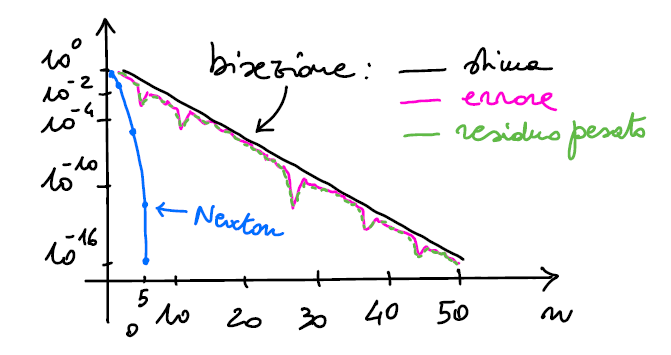
\includegraphics{foto/pagina25}
\end{center}
Perché il metodo di Newton è così veloce? Per capirlo, dobbiamo analizzare l'errore, in particolare quale relazione leghi $e_{n+1}$ con $e_n$ (dove come al solito $e_n=\abs{\,x_n-\xi\,})$\\\\
Enunciamo il risultato sul comportamento dell'errore come teorema, che poi dimostreremo.

\subsection{TEOREMA (sulla velocità di convergenza del metodo di Newton)}
\begin{center}
    \fbox{\begin{minipage}[t]{15cm}%
        Sia $f \in C^2 [a,b]$ e si assuma di essere in ipotesi che garantiscano la convergenza del metodo di Newton e $\xi \in [a,b] : f(\xi) = 0$; sia inoltre $\{x_n\} \subset [c,d] \subseteq [a,b]$ con $f'(x) \neq 0$ $\forall x\in [c,d]$
        allora 
        \[e_{n+1} \le c\ e_n^2, \quad n\ge0, \quad c = \frac{1}{2} \cdot \frac{M_2}{m_1}\]
        \[\text{con } M_2 = \max_{x\in[c,d]}\abs{\,f''(x)\,}, \quad m_1 = \min_{x\in[c,d]}\abs{\,f'(x)\,} > 0\]
    \end{minipage}}
\end{center}
Prima di dimostrare questa disuguaglianza, osserviamo che:
\begin{enumerate}[label=\roman*)]
\item l'ipotesi $\{x_n\} \subset [c,d]$ con $f'(x)\neq0$ in $[c,d]$, come abbiamo già visto nell'analisi del residuo pesato col metodo di bisezione, ci assicura che lo zero $\xi$ è semplice, cioè $f'(\xi) \neq 0$

\item tale ipotesi è soddisfatta ad esempio nelle condizioni del teorema di convergenza dimostrato prima con $[c,d] = [\xi, b]$ nei casi 1) e 3), $[c,d] = [a,\xi]$ nei casi 2) e 4).
\end{enumerate}

\begin{proof}[\unskip\nopunct]
\textbf{Dimostrazione}\\
Applicando la formula di Taylor centrata in $x_n$ e calcolata in $\xi $ , con resto del secondo ordine in forma di Lagrange
\[f(\xi)=f(x_n)+f'(x_n)(\xi-x_n)+\frac{f''(z_n)}{2}(\xi-x_n)^2\]
dove $z_n\in int(x_n,\xi)\subset [c,d]$ e $f(\xi)=0$, da cui 
\[-\frac{f(x_n)}{f'(x_n)}=\xi-x_n+\frac{f''(z_n)}{2f'(x_n)}(\xi-x_n)^2\]
Ma dalla definizione del metodo
\[-\frac{f(x_n)}{f'(x_n)}=x_{n+1}-x_n\]
che inserita nella formula di Taylor porta a 
\[x_{n+1}-x_n=\xi-x_n+\frac{f''(z_n)}{2f'(x_n)}(\xi-x_n)^2\]
ovvero mettendo i moduli
\[e_{n+1}=\abs{\,x_{n+1}-\xi\,}=c_ne_n^2 \quad \text{con} \quad c_n=\frac{1}{2}\frac{\abs{\,f''(z_n)\,}}{\abs{\,f'(x_n)\,}}\]
La successione $\{c_n\}$ è limitata, infatti 
\[\abs{\,f''(z_n)\,}\leq \max_{x \in [c,d]}\abs{\,f''(x)\,}=M_2\]
applicando il teorema di Weierstrass sull'esistenza di massimo e minimo assoluti a $ \abs{\,f''(x)\,}\in C[c,d]$.\\
D'altra parte, applicando lo stesso teorema a  $ \abs{\,f'(x)\,}\in C[c,d]$ abbiamo che 
\[m_1=\min_{x \in [c,d]}\abs{\,f'(x)\,}>0\] 
(perché $\exists \ \overline{x}: m_1=\abs{\,f'(\overline{x})\,} $  e    $f'(\overline{x})\neq 0$   )\\
Otteniamo quindi $\abs{\,f'(x_n)\,}\geq m_1>0$ e infine $c_n \leq \frac{1}{2}\frac{M_2}{m_1}=c$. 
\newline 
\end{proof}

\subsection{Confronto con bisezione}
La relazione di tipo \uline{quadratico}
\[\fbox{$e_{n+1}\leq ce_n^2$}\]
è la chiave per spiegare la velocità di convergenza del metodo di Newton, perché ci dice in sostanza che \uline{l'errore  al passo n+1} è maggiorato da una quantità \uline{proporzionale} (con costante di proporzionalità non dipendente da $n$) al \uline{quadrato} dell'\uline{errore al passo $n$} \\
Si noti la notevole differenza col metodo di bisezione, dove la relazione tra $e_{n+1}$ ed $e_n$ è lineare ($e_{n+1} \approx \frac{1}{2} e_n$, in media).
Per apprezzare l'effetto della relazione quadratica, prima di tutto osserviamo che
\[ ce_{n+1} \leq c \cdot c \cdot e_{n}^2 = ( ce_n)^2\]
Ora, fissiamo $\theta \in (0,1)$:\\
siccome abbiamo assunto che il metodo sia convergente, $ce_n\rightarrow0,\ n\rightarrow\infty$ e quindi $\exists \,\overline{n} : ce_n \leq \theta \quad \forall n \geq \overline{n}$\\
(con $\overline{n}$ dipendente da $\theta$). Applicando la disuguaglianza  $ce_{n+1} \leq (ce_n)^2 \ per \ n \geq \overline{n}$ : 
\[\begin{split}
    ce_{\overline{n}+1} & \le (ce_{\overline{n}})^2 \le \theta^2 \\
    ce_{\overline{n}+2} & \le (ce_{\overline{n}+1})^2\le \left(\theta^2\right)^2 = \theta^4 \\
    ce_{\overline{n}+3} & \le (ce_{\overline{n}+2})^2 \le \left(\theta^4\right)^2 = \theta^8 \\
    \dotso \\
    ce_{\overline{n}+k}& \le (ce_{\overline{n}+k-1})^2 \le \left(\theta^{2^{k-1}}\right)^2 = \theta^{2^k}
\end{split} \]
Adesso, solo per fissare le idee nel confronto col metodo di bisezione, prendiamo $\theta=\frac{1}{2}$. \\
Otteniamo, dopo $k$ iterazioni di Newton a partire da $\overline{n}$ \\
\[e^{\scalebox{.6}{$Newt$}}_{\overline{n}+k}\leq\frac{1}{c}\cdot\left(\frac{1}{2}\right)^{2^k}\]
mentre con $k$ iterazioni del metodo di bisezione 
\[ e^{bisez}_{k}\lesssim \left(\frac{1}{2}\right)^k e_{0}^{bisez}\]
Il confronto sulle $k$ iterazioni va fatto guardando gli esponenti
di $\frac{1}{2}$: nella bisezione l'esponente è $k$ ( cioè cresce linearmente in $k$), con Newton invece l'esponente è $2^k$ (cioè cresce \uline{esponenzialmente} in $k$)\\
Ad esempio per $k=6$ nella stima per la bisezione compare
\[\left(\frac{1}{2}\right)^{6}=\frac{1}{64}\approx 1.6\cdot10^{-2}\]
mentre nella stima per Newton
\[\left(\frac{1}{2}\right)^{2^6}=\left(\frac{1}{2}\right)^{64}\approx 5\cdot10^{-20}\]
Ribadiamo che $\theta=\frac{1}{2}$ è stato scelto arbitrariamente solo per fare un confronto diretto col metodo di bisezione, dove il fattore di riduzione $\frac{1}{2}$ è intrinseco nella costruzione; nel caso del metodo di Newton (per zeri semplici) possiamo dire sostanzialmente che non appena $ce_n<1$ si innesca una riduzione rapidissima dell'errore, di tipo ``quadrati successivi", che viene detta \uline{CONVERGENZA QUADRATICA} (concetto che formalizzeremo nella prossima lezione)
\newpage
